\documentclass[14pt]{beamer}

\usetheme{Madrid}

% Add frame numbers
\setbeamertemplate{page number in head/foot}[framenumber]

\usepackage{amsmath, amssymb}
\usepackage{tikz}
\usepackage{bm}
\usepackage{outlines}   % For multilevel lists using the outline environment
\usepackage{natbib}
\usepackage{subcaption}

\renewcommand*{\bibfont}{\scriptsize}

\newcommand{\CMA}{Causal Mediation Analysis}

\newcommand{\bE}{\mathbb{E}}
\newcommand{\bF}{\mathbb{F}}
\newcommand{\bG}{\mathbb{G}}

\newcommand{\GLMMs}{Mixed-Effects Models}

\title[]{Adaptive Pareto Smoothed Importance Sampling}
\author{William Ruth}
\institute[]{Joint work with Payman Nickchi}
\date{\vspace{-3cm}}
% \titlegraphic{
\includegraphics[width=2cm]{../Logos/CANSSI_Logo.png} \hspace{2cm} 
\includegraphics[width=4cm]{../Logos/Logo_UdeM-CMJN.jpg}}


\begin{document}

\begin{frame}
    \titlepage
\end{frame}

\begin{frame}
    \centering
    
\includegraphics[height=0.9\textheight]{Figures/RichCon2.png}
\end{frame}

\begin{frame}{Introduction}
    \begin{outline}
        \1 Importance sampling \newline
        \1 Measuring performance \newline
        \1 Improving performance
            \2 Modifications
            \2 Optimization
    \end{outline}
\end{frame}


\begin{frame}{Importance Sampling}
    \begin{outline}
        \1 Need to compute an expected value
            \2 $\bE_F \varphi(X)$
        \1 Can't do the sum/integral \newline

        \1 Monte Carlo approximation
            \2 Simulating from $F$ might be hard
    \end{outline}
    \begin{equation*}
    \end{equation*}
\end{frame}

\begin{frame}{Importance Sampling}
    \begin{outline}
        \1 Introduce ``proposal distribution'', $G$:
    \end{outline}
    \begin{align*}
        \bE_F \varphi(X) &=  \bE_G \left[ \varphi(X) \cdot \frac{f(X)}{g(X)} \right] \\
        &=  \bE_G \left[ \varphi(X) \cdot w(X) \right]
    \end{align*}
    \begin{outline}
        \1 $G$ can be nearly anything*
            \2 *Some choices will be better than others
    \end{outline}
\end{frame}

\begin{frame}{Example: Mystery Target}
    \begin{outline}
        \1 $f$ unknown, but can be evaluated 
        \1 $\varphi(X) = X^2$ \newline

        \1 Try some proposals:
            \2 $G_1 \sim N(0.1,1)$
            \2 $G_2 \sim N(1.5,1)$ \newline
        \1 Use $M=1000$ samples from proposal
            \2 $\hat{\bE}_1 = 1.07$, $SE = 0.05$
            \2 $\hat{\bE}_2 = 1.04$, $SE = 0.19$
    \end{outline}    
\end{frame}

\begin{frame}{Example: Mystery Target}
    \centering
    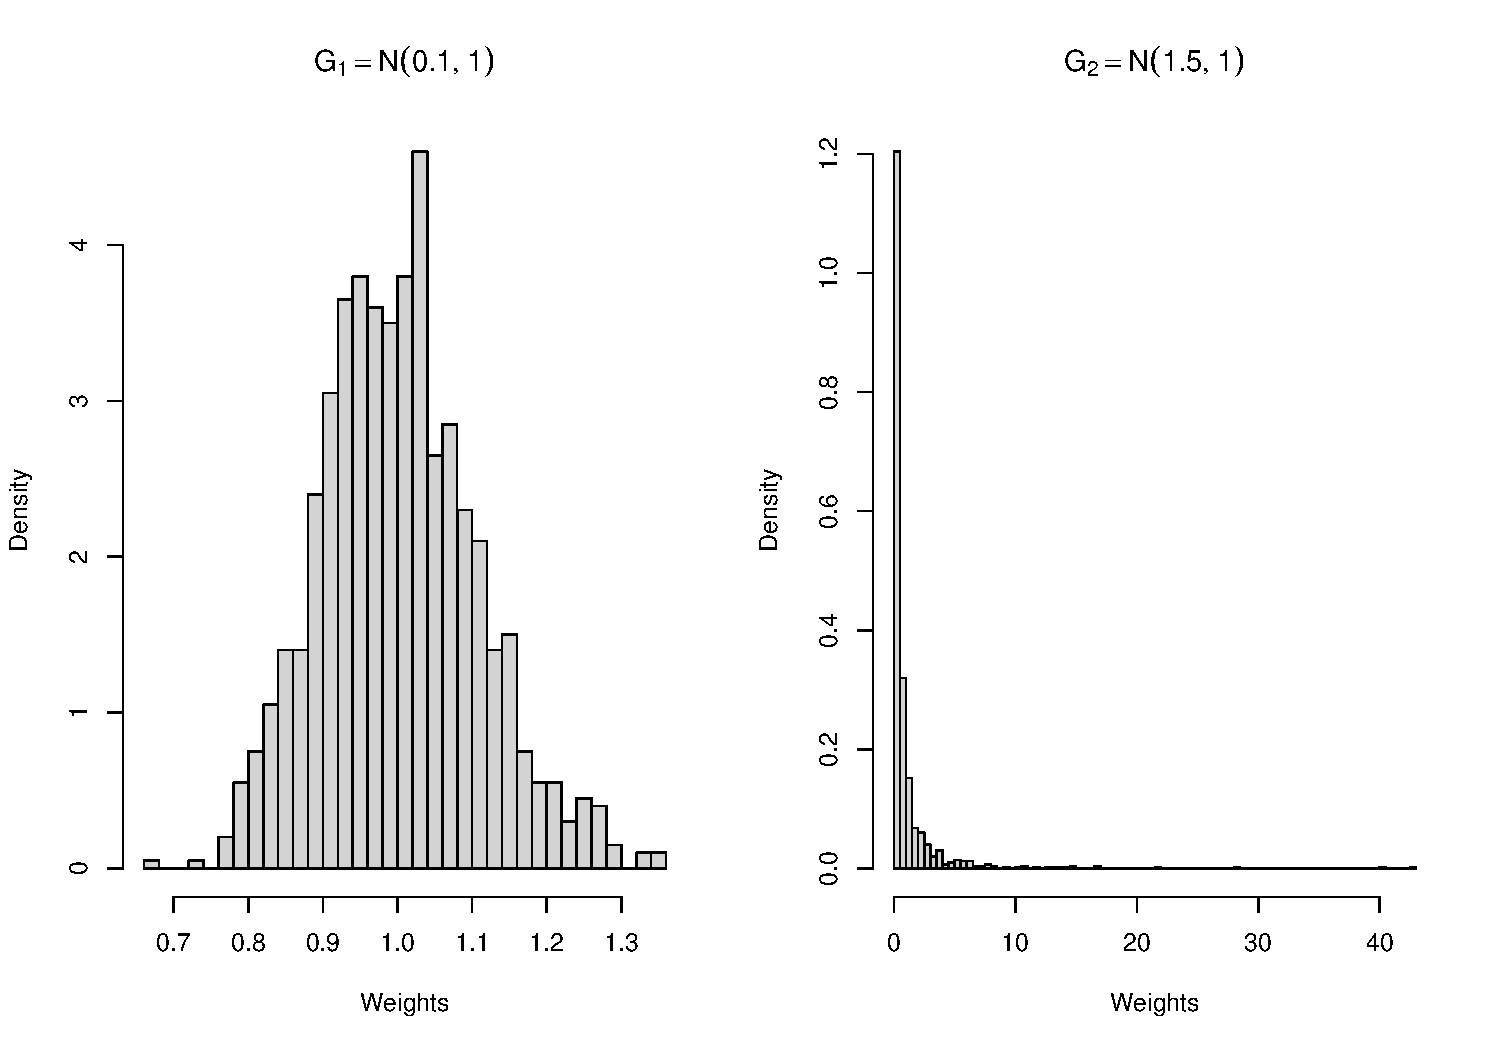
\includegraphics[height=0.9\textheight, width=0.9\textwidth, keepaspectratio]{Figures/Wt Hist.pdf}
\end{frame}

\begin{frame}{Importance Sampling}
    \begin{outline}
        \1 We can make this difference precise
        \1 ``Effective Sample Size'':
    \end{outline}
    \begin{gather*}
        ESS = \frac{\left[\sum_i w(X_i)\right]^2}{\sum_i w(X_i)^2}
    \end{gather*}
\end{frame}

\begin{frame}{Example: Mystery Target}
    \centering
    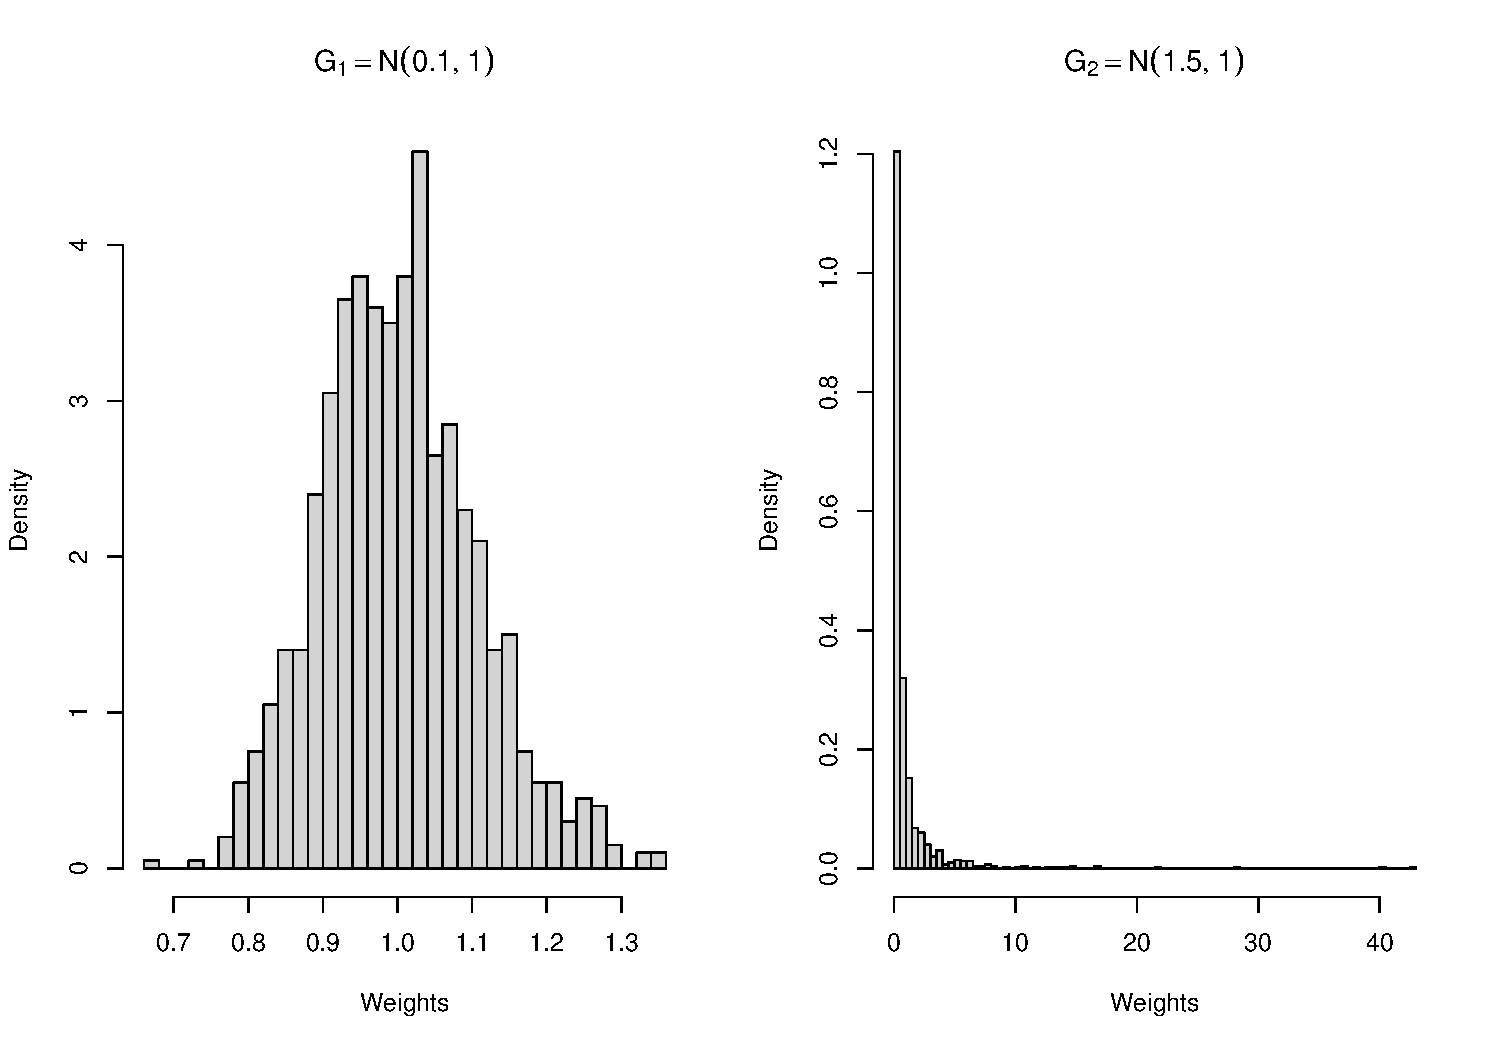
\includegraphics[height=0.7\textheight, width=0.9\textwidth, keepaspectratio]{Figures/Wt Hist.pdf} \newline
    \begin{outline}
        $ESS_1 \approx 989$ \hspace{2.5cm} $ESS_2 \approx 131$
    \end{outline}
\end{frame}

\begin{frame}{Importance Sampling}
    \begin{outline}
        \1 Problem: Low ESS $\rightarrow$ hard to estimate means \newline
        \1 But ESS is based on means
            \2 \citep{Cha18}
    \end{outline}
\end{frame}

% \begin{frame}{Importance Sampling}
%     \begin{outline}
%         \1 Consider $\varphi(X) = X$
%             \2 I.e. $\bE_F \varphi(X) = \bE_F(X)$ \newline
%         \1 $\hat{\bE} = \sum_i \frac{X_i w(X_i)}{M}$, $X_i \overset{\mathrm{iid}}{\sim} G$ \newline

%         \1 The variance of our estimator is \left( \sum_i w(X_i)^2 \right)
%     \end{outline}
% \end{frame}


\begin{frame}{Improving IS}
    \begin{outline}
        \1 Choose a good proposal \newline
        
        \1 Modify large weights        
            \2 Truncated IS
            \2 Pareto Smoothed IS
    \end{outline}
\end{frame}

\begin{frame}{Improving IS}
    \begin{outline}
        \1 Truncated Importance Sampling:
            \2 \citep{Ion08} \newline
    \end{outline}

    \setbeamertemplate{enumerate items}[default]
    \begin{enumerate}
        \item Choose a threshold
        \item Set any weights above threshold equal to threshold
    \end{enumerate}
\end{frame}

\begin{frame}{Example: Mystery Target}
    \centering
    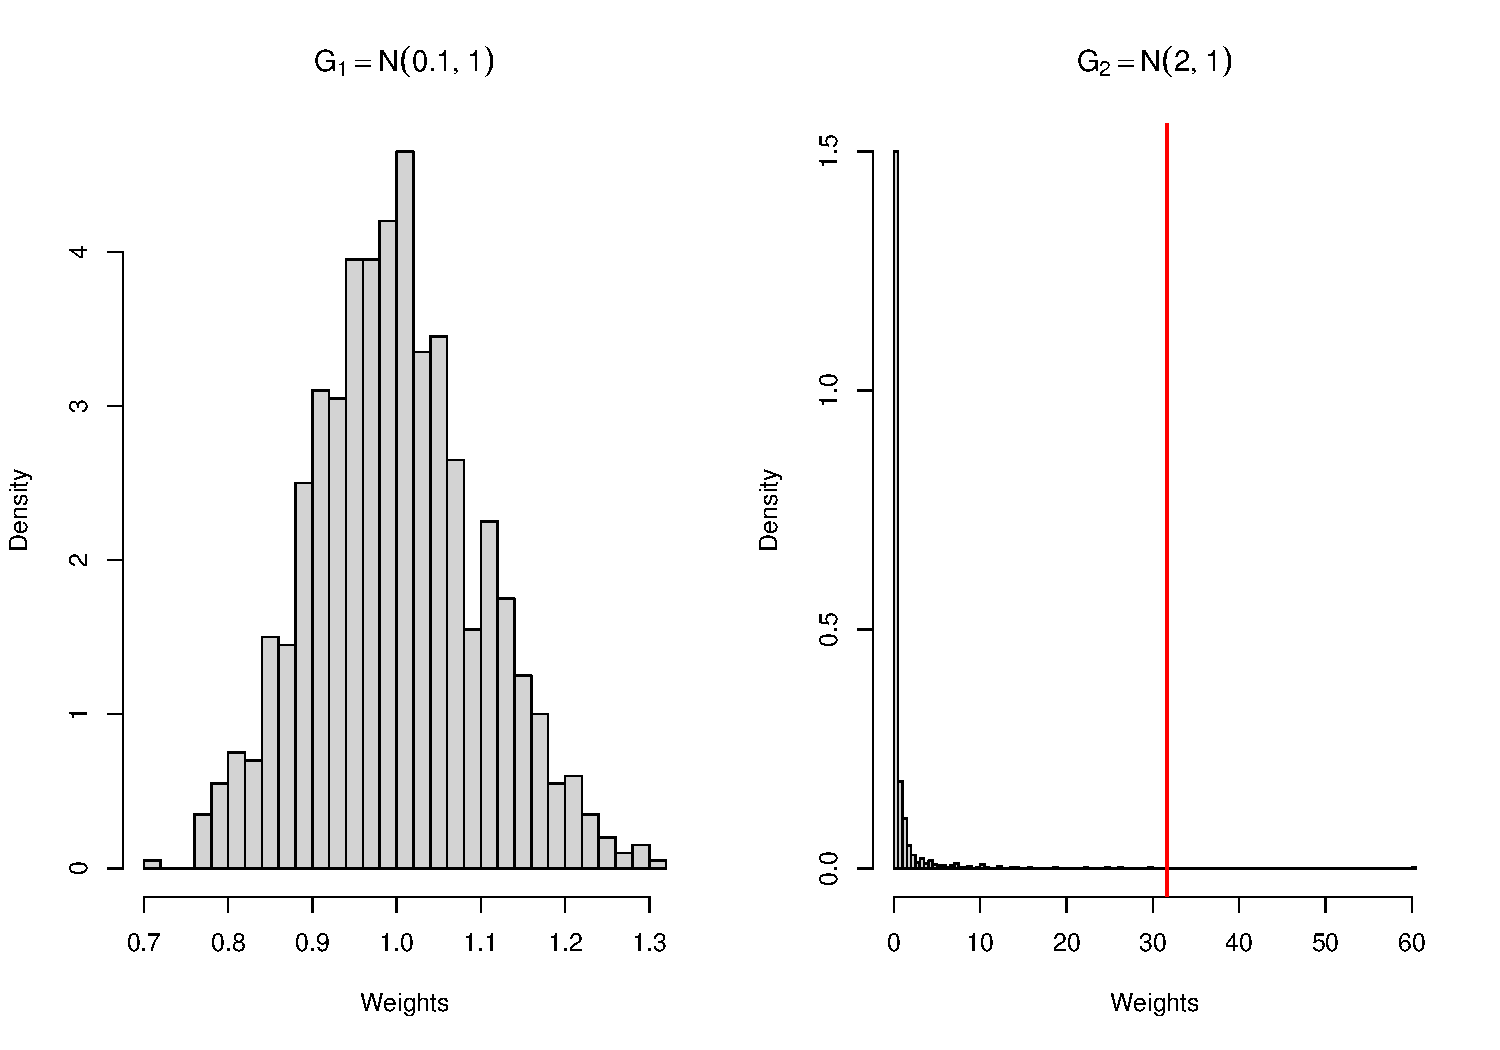
\includegraphics[height=0.9\textheight, width=0.9\textwidth, keepaspectratio]{Figures/Wt Hist - Thresh.pdf}
\end{frame}

% \begin{frame}{Example: Mystery Target}
%     \centering
%     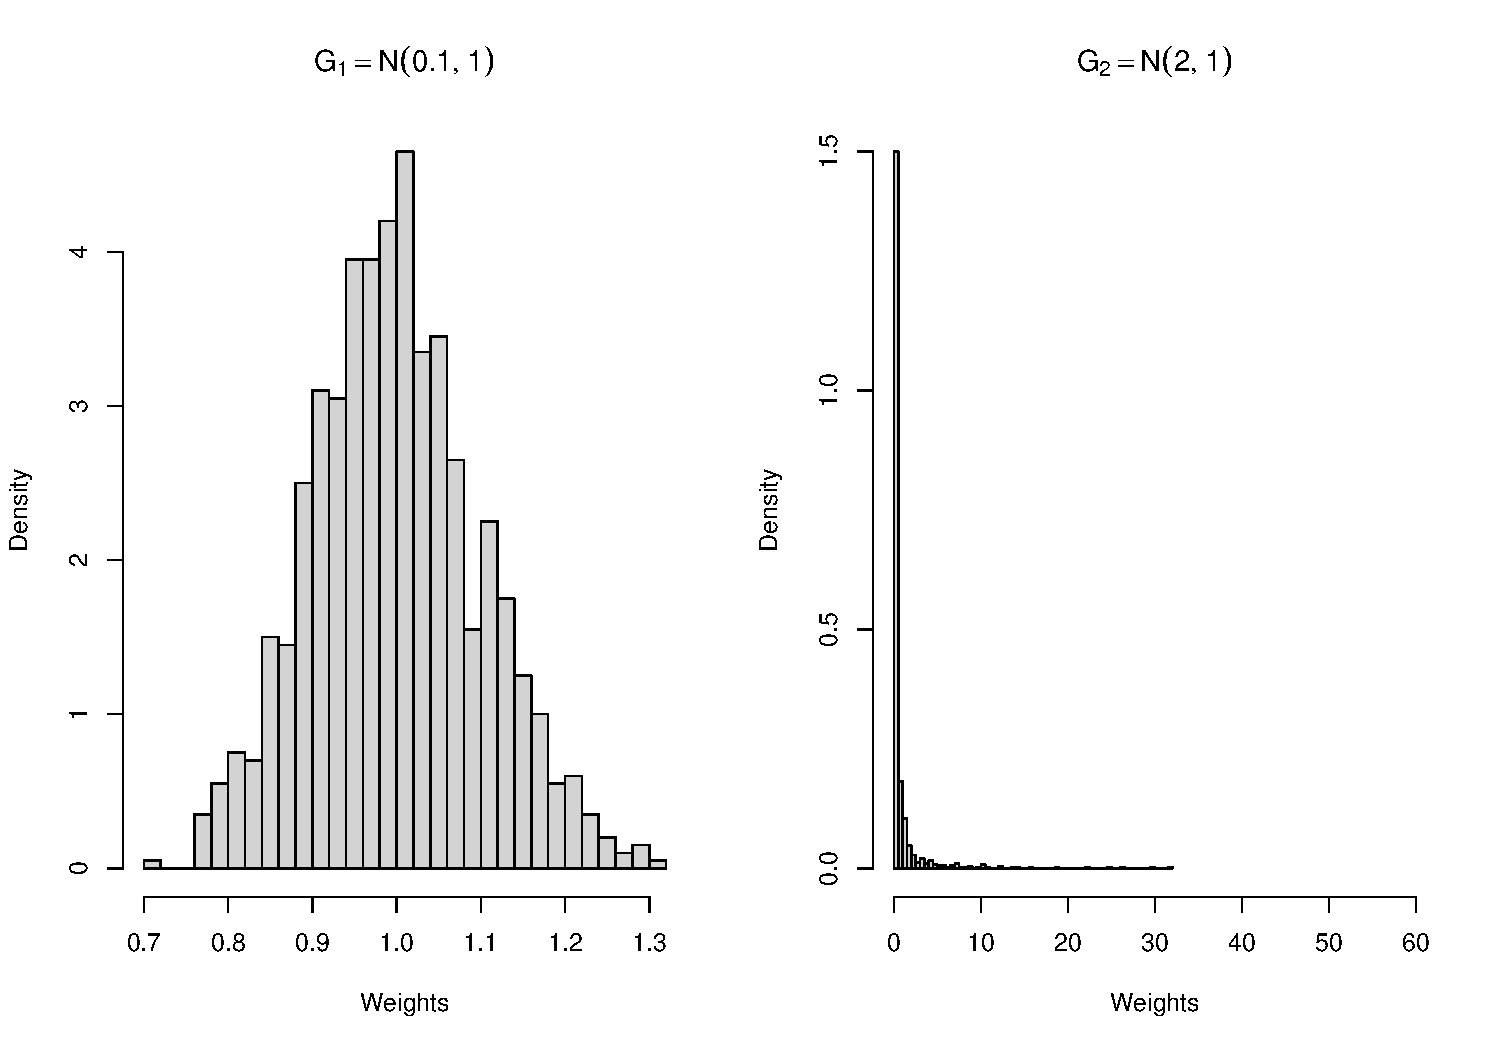
\includegraphics[height=0.9\textheight, width=0.9\textwidth, keepaspectratio]{Figures/Wt Hist - Trunc.pdf}
% \end{frame}

\begin{frame}{Example: Mystery Target}
    \centering
    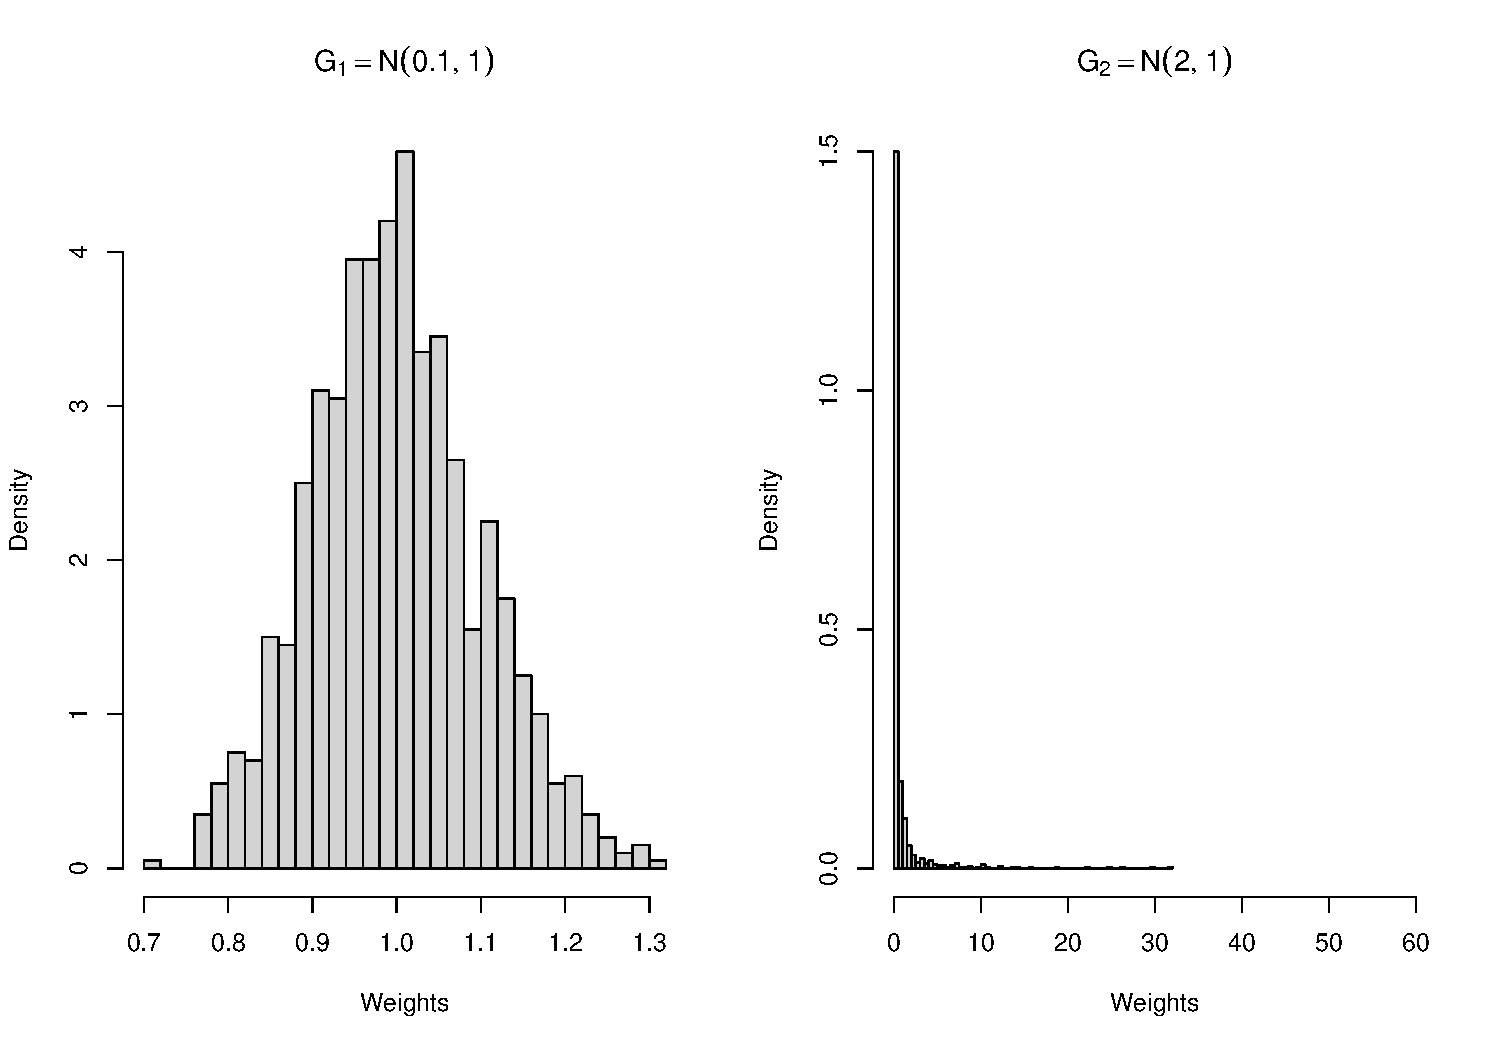
\includegraphics[height=0.7\textheight, width=0.9\textwidth, keepaspectratio]{Figures/Wt Hist - Trunc.pdf} \newline
    \begin{outline}
        $ESS_1 \approx 989$ \hspace{2.5cm} $ESS_2 \approx 131$\\
        $ESS_1^{(\mathrm{trunc})} \approx 989$ \hspace{2.5cm} $ESS_2^{(\mathrm{trunc})} \approx 144$
    \end{outline}
\end{frame}


\begin{frame}{Improving IS}
    \begin{outline}
    \1 Pareto Smoothed Importance Sampling:
        \2 \citep{Veh22} \newline
    \end{outline}

    \setbeamertemplate{enumerate items}[default]
    \begin{enumerate}
    \item Choose a threshold
        \begin{itemize}
            \item Weights above threshold represent tail of their dist.
        \end{itemize}
    \item Approximate tail with Generalized Pareto Dist.
    \begin{itemize}
        \item Fit GPD to weights above threshold
        \item \citep{Zha09}
    \end{itemize}
    \item Replace large weights with quantiles of fitted GPD
    \end{enumerate}
\end{frame}

\begin{frame}{Example: Mystery Target}
    \centering
    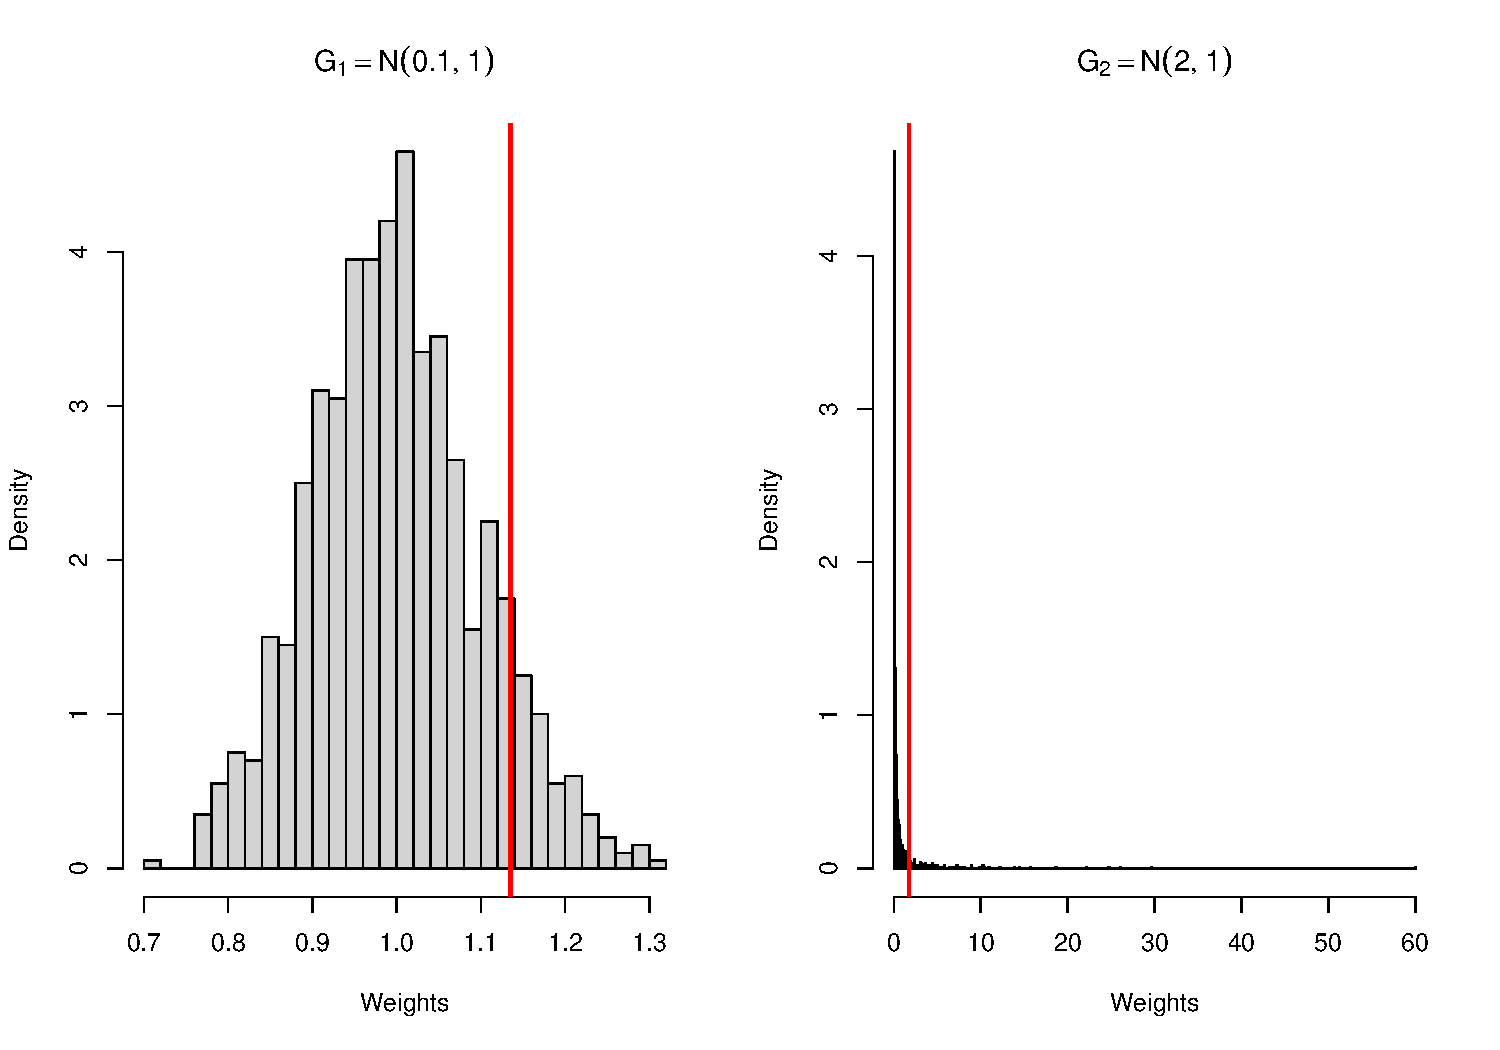
\includegraphics[height=0.9\textheight, width=0.9\textwidth, keepaspectratio]{Figures/Wt Hist - Pareto Thresh.pdf}
\end{frame}

\begin{frame}{Example: Mystery Target}
    \centering
    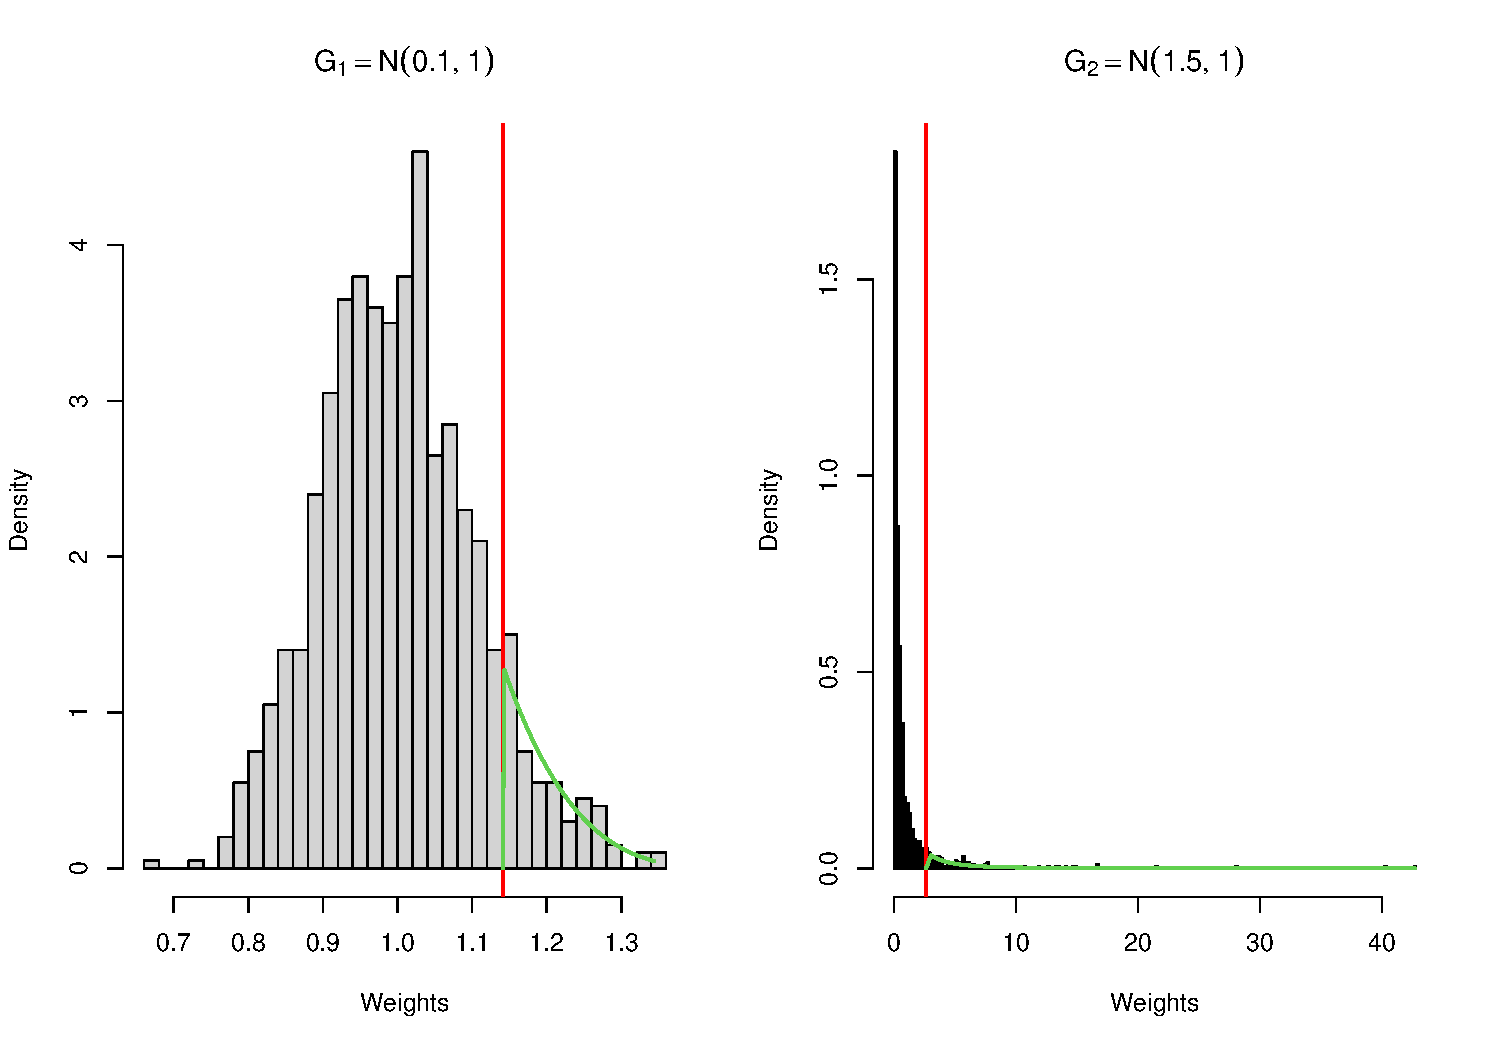
\includegraphics[height=0.9\textheight, width=0.9\textwidth, keepaspectratio]{Figures/Wt Hist - Pareto Dens.pdf}
\end{frame}

\begin{frame}{Example: Mystery Target}
    \centering
    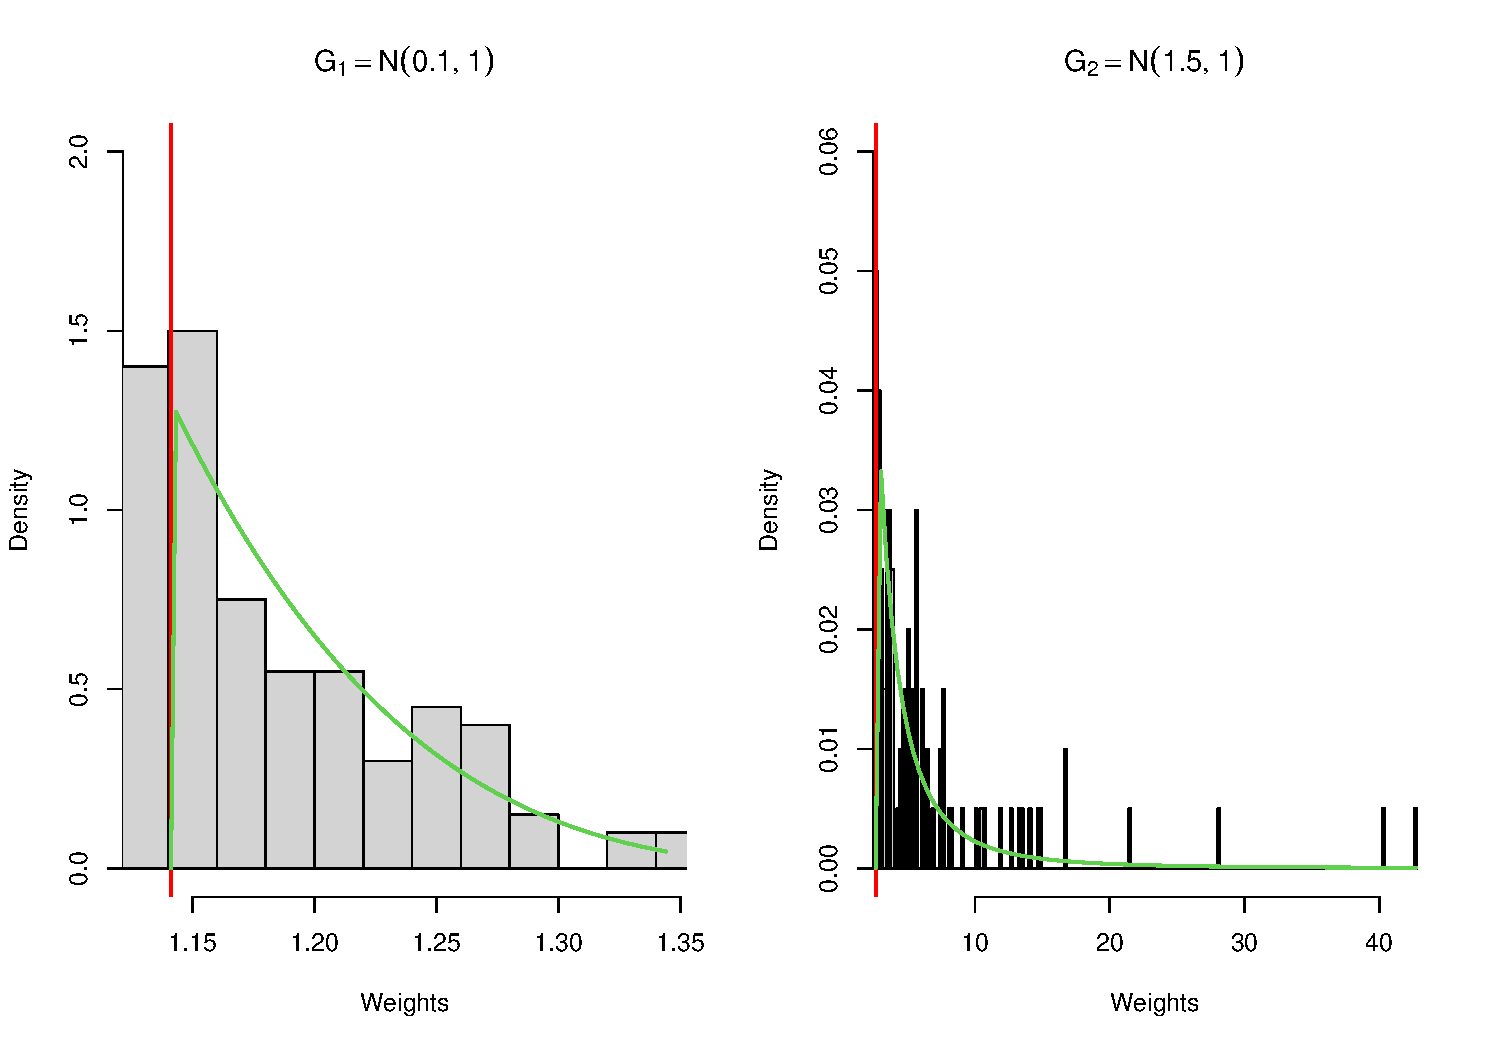
\includegraphics[height=0.9\textheight, width=0.9\textwidth, keepaspectratio]{Figures/Wt Hist - Pareto Dens Zoom.pdf}
\end{frame}

\begin{frame}{Example: Mystery Target}
    \centering
    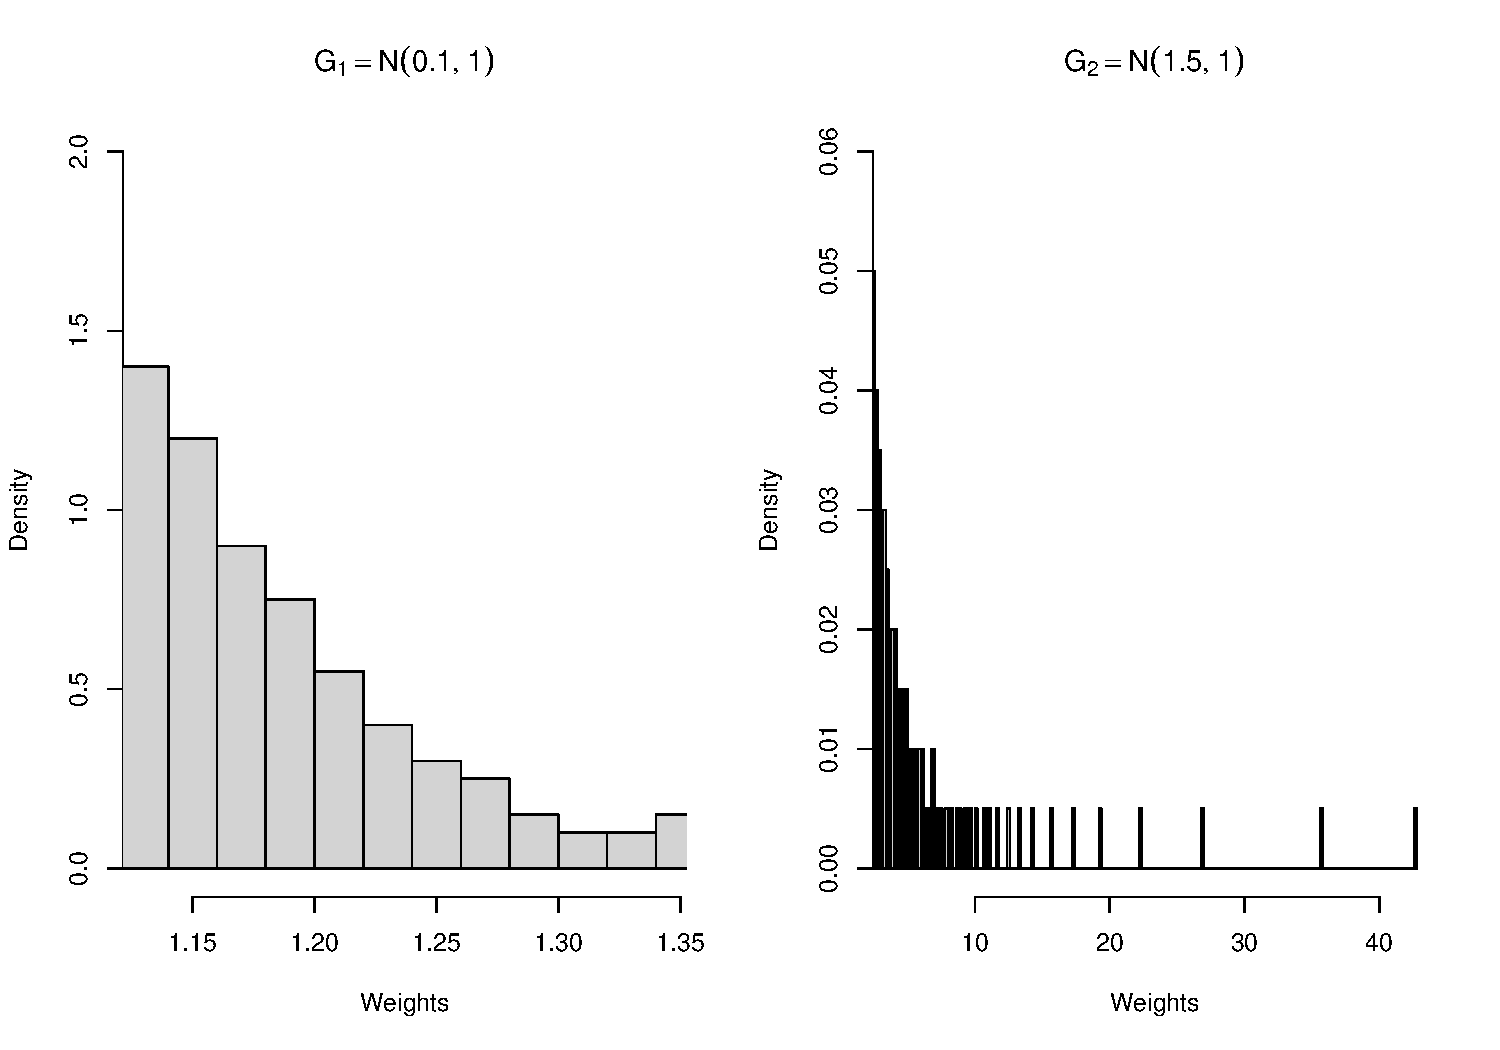
\includegraphics[height=0.9\textheight, width=0.9\textwidth, keepaspectratio]{Figures/Wt Hist - Pareto Smooth Zoom.pdf}
\end{frame}

\begin{frame}{Example: Mystery Target}
    \centering
    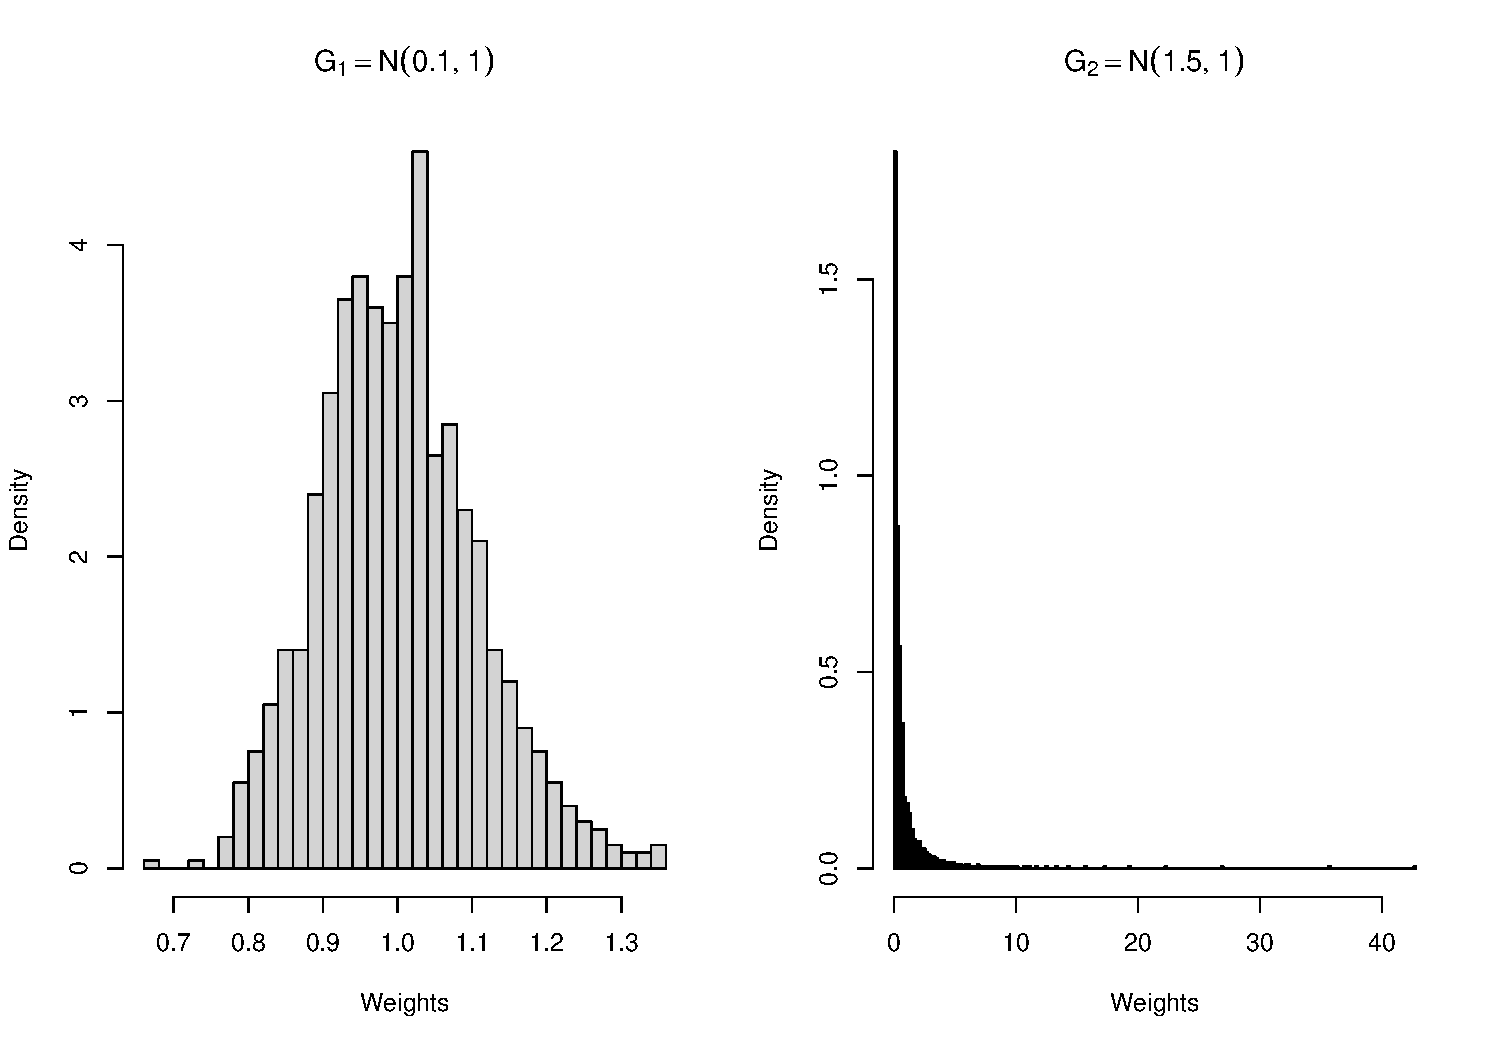
\includegraphics[height=0.5\textheight, width=0.9\textwidth, keepaspectratio]{Figures/Wt Hist - Pareto Smooth.pdf}\newline
    \begin{outline}
        $ESS_1 \approx 989$ \hspace{2.5cm} $ESS_2 \approx 131$\\
        $ESS_1^{(\mathrm{trunc})} \approx 989$ \hspace{2.5cm} $ESS_2^{(\mathrm{trunc})} \approx 144$\\
        $ESS_1^{(\mathrm{PS})} \approx 989$ \hspace{2.5cm} $ESS_2^{(\mathrm{PS})} \approx 135$
    \end{outline}
\end{frame}


\begin{frame}{Adaptive IS}
    \begin{outline}
        \1 Alternative approach: directly optimize ESS \newline

        \1 Adaptive Importance Sampling: 
            \2 \citep{Aky21} \newline
    \end{outline}

    \begin{enumerate}
        \setbeamertemplate{enumerate items}[default]
        \item Choose a (parametric) family of proposals
        \item Iteratively update the proposal to maximize ESS
    \end{enumerate}
\end{frame}

\begin{frame}{Stochastic Approximation}
    \begin{outline}
        \1 Actually, we want to maximize a population-level analog: $\overline{ESS}$ \newline

        \1 If we had $\overline{ESS}$, we would do gradient ascent
            \2 $\theta_{k+1} = \theta_k + \alpha \nabla \overline{ESS}(\theta_k)$ \newline

        \1 Instead, do gradient ascent on $ESS$
            \2 $\hat{\theta}_{k+1} = \hat{\theta}_k + \alpha_k \nabla ESS(\hat{\theta}_k)$
    \end{outline}
\end{frame}

\begin{frame}{Stochastic Approximation}
    \begin{outline}
        \1 Stochastic approximation
            \2 \citep{Rob51} \newline

        \1 Finite difference approximation to  $\nabla ESS$
            \2 \citep{Kie52}
    \end{outline}
\end{frame}


\begin{frame}{Example: Mystery Target}
    \centering
    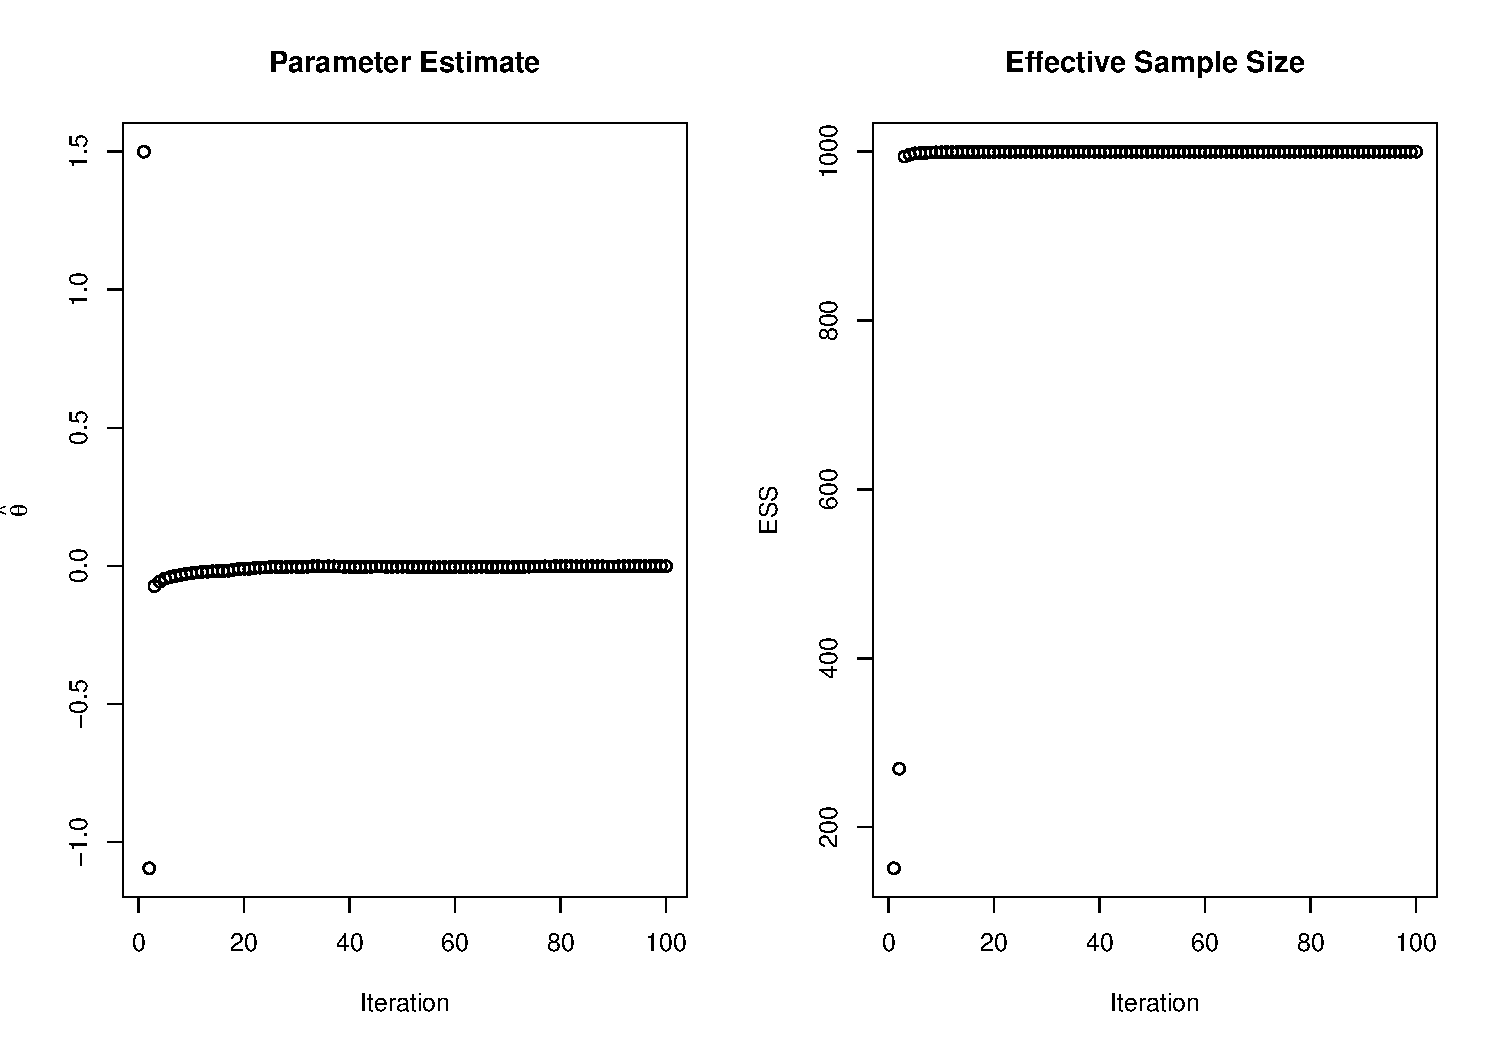
\includegraphics[height=0.7\textheight, width=0.9\textwidth, keepaspectratio]{Figures/ESS traj.pdf} \newline
    \begin{outline}
        $\hat{\theta}_\mathrm{end}^{(ESS)} \approx -8 \times 10^{-4}$ \hspace{1cm} $ESS_\mathrm{end} \approx 1000 - (7 \times 10^{-4})$
    \end{outline}
\end{frame}


\begin{frame}{Our Method}
    \begin{outline}
        \1 Recall: Be careful using IS means to diagnose IS \newline
        
        \1 \citeauthor{Veh22} give an alternative
            \2 Shape parameter of fitted tail distribution, $\hat{k}$
    \end{outline}
\end{frame}

\begin{frame}{Our Method}
    \begin{outline}
        \1 Use diagnostic as objective function \newline

        \1 Apply stochastic approximation to minimize $\hat{k}$
            \2 More precisely, $k(\theta)$
    \end{outline}
\end{frame}


\begin{frame}{Example: Mystery Target}
    \centering
    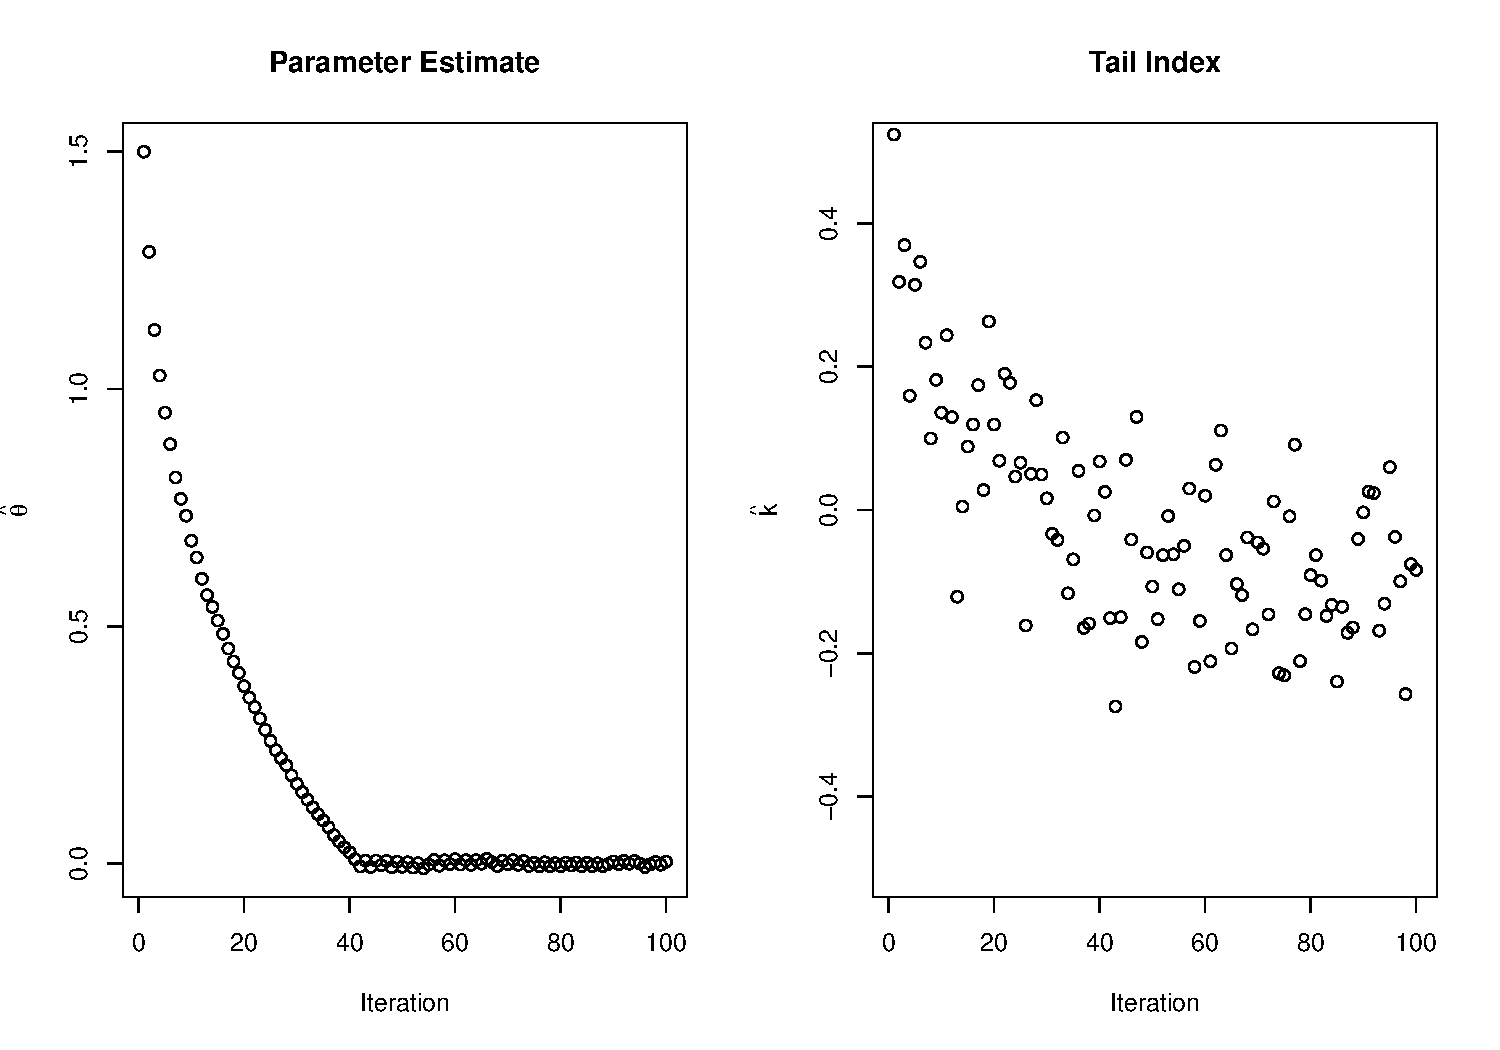
\includegraphics[height=0.7\textheight, width=0.9\textwidth, keepaspectratio]{Figures/PS traj.pdf} \newline
    \begin{outline}
        $\hat{\theta}_\mathrm{end}^{(PS)} \approx 4 \times 10^{-3}$ \hspace{5cm}
    \end{outline}
\end{frame}

\begin{frame}{Example: Mystery Target}
    \centering
    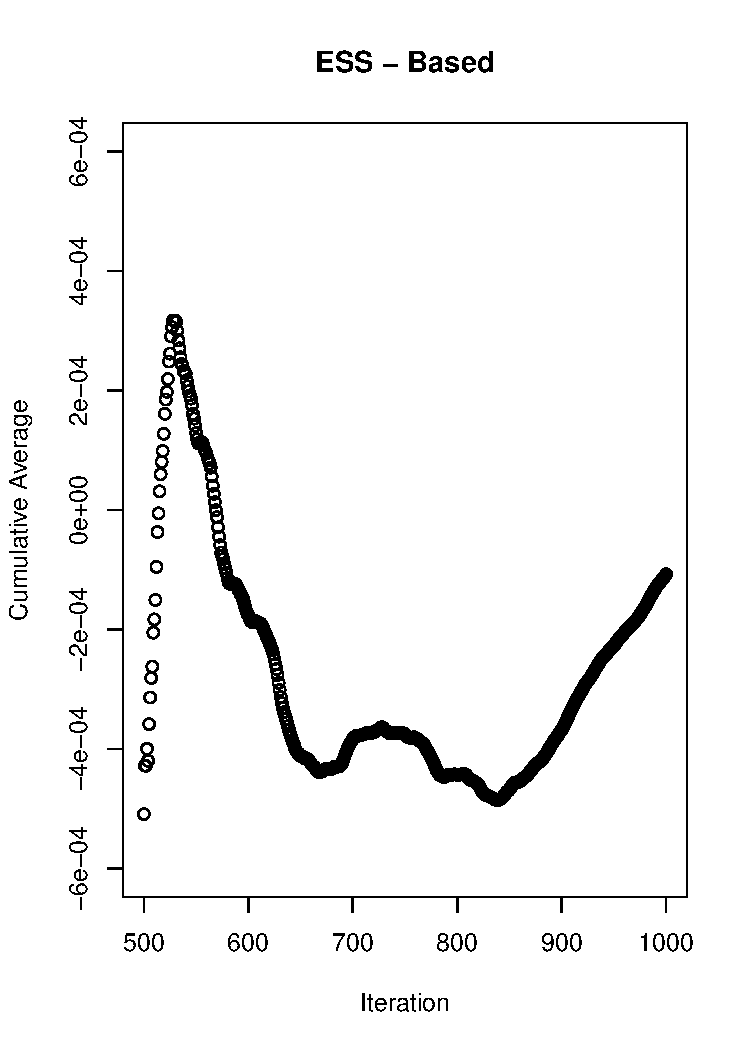
\includegraphics[height=0.7\textheight, width=0.45\textwidth]{Figures/ESS mean traj.pdf}%
    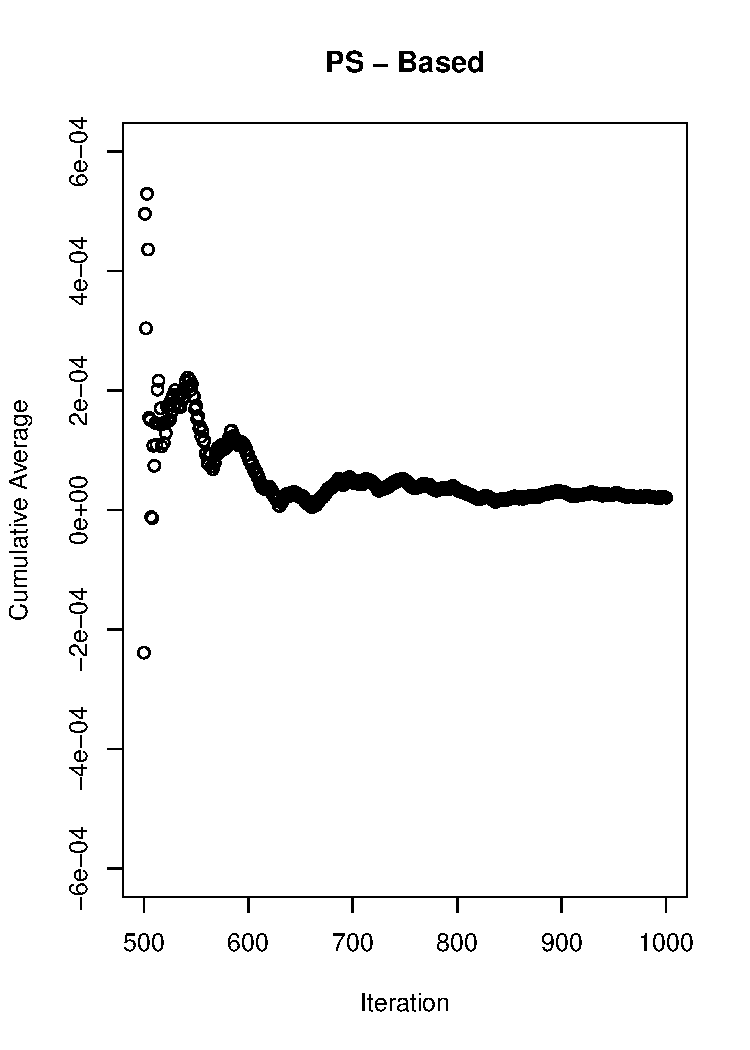
\includegraphics[height=0.7\textheight, width=0.45\textwidth]{Figures/PS mean traj.pdf} \newline
    \begin{outline}
        $\bar{\theta}_\mathrm{end}^{(ESS)} \approx -1 \times 10^{-4}$ \hspace{1.5cm} $\bar{\theta}_\mathrm{end}^{(PS)} \approx 2 \times 10^{-5}$
    \end{outline}
\end{frame}


\begin{frame}{Recap}
    \begin{outline}
        \1 Importance sampling and extensions
            \2 Truncation
            \2 Pareto Smoothing \newline
        
        \1 Diagnostics for importance sampling
            \2 Effective sample size
            \2 Pareto tail index \newline

        \1 Adaptive importance sampling
            \2 Stochastic approximation
    \end{outline}
\end{frame}


% \begin{frame}{Acknowledgements}
%     Collaborators:
%     \begin{itemize}
%         \item Payman Nickchi
%         \item Richard Lockhart
%     \end{itemize}

%     Funding:
%     \begin{itemize}
%         \item Canadian Statistical Sciences Institute
%     \end{itemize}
% \end{frame}

\begin{frame}{Acknowledgements}
    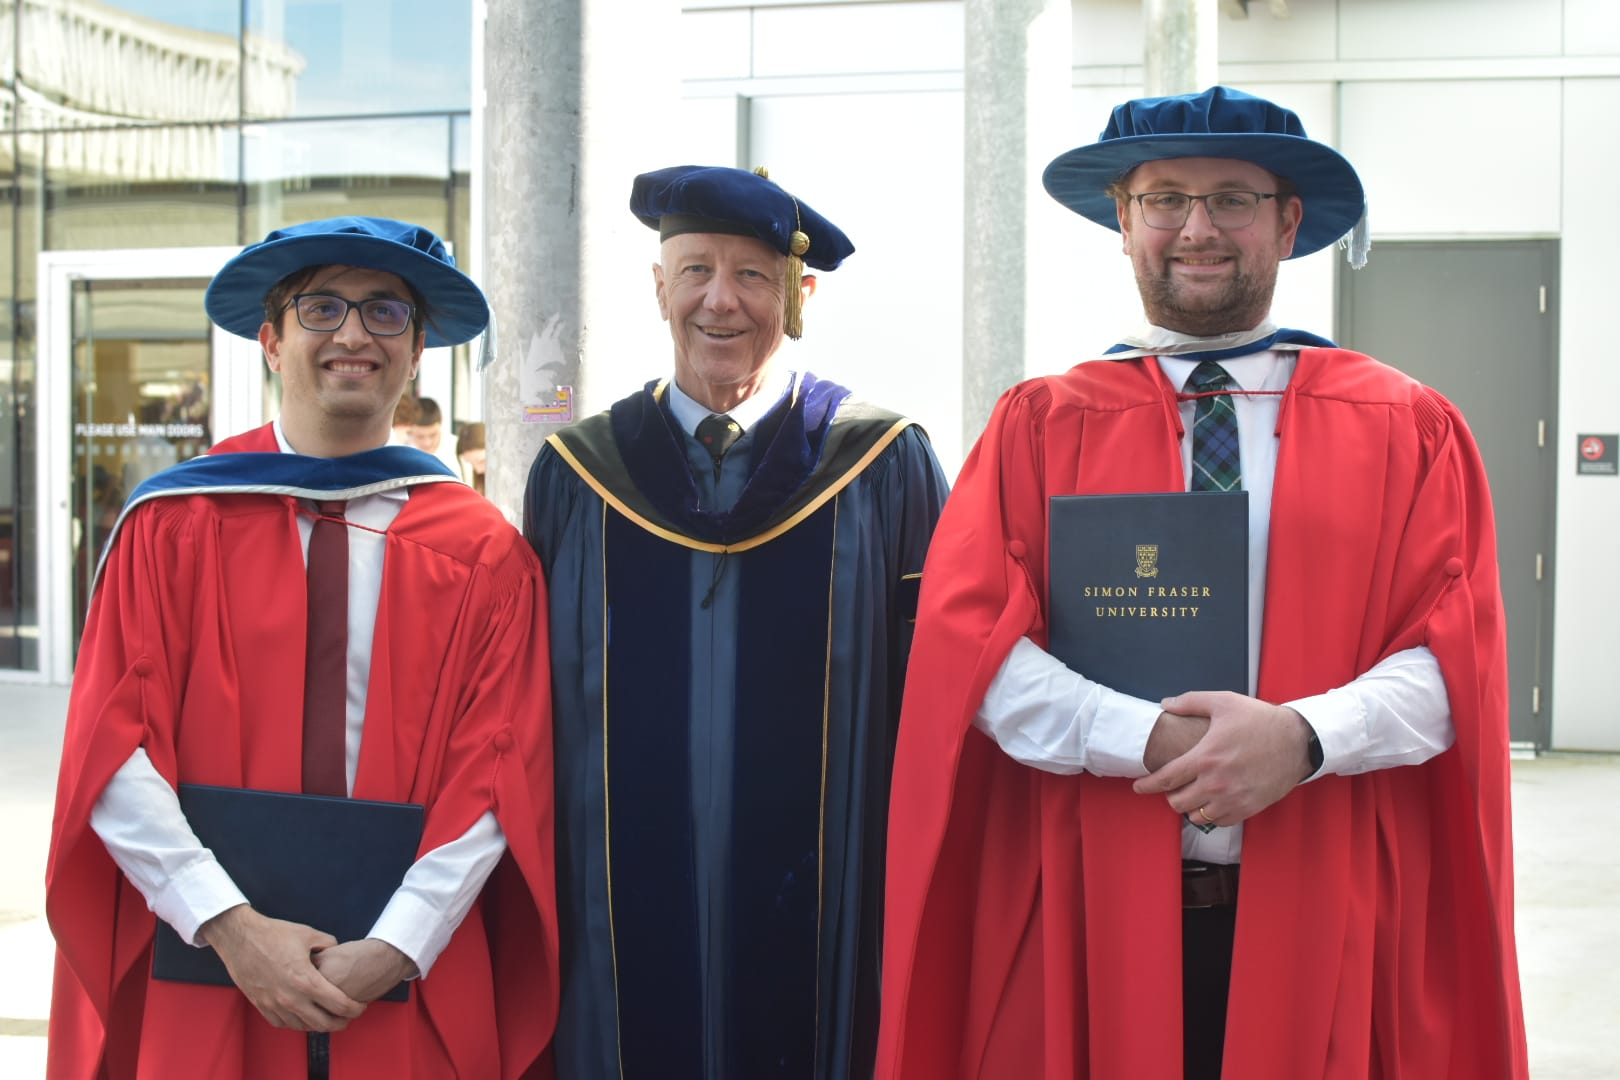
\includegraphics[width=\textwidth]{Figures/Convocation Image.jpg}
\end{frame}

\begin{frame}
    \centering
    \Huge Thank You
\end{frame}

\begin{frame}{Some References}
    \bibliographystyle{apalike}
    \bibliography{Refs}
\end{frame}

\end{document}
